\documentclass[aspectratio=169]{../latex_main/tntbeamer}  % you can pass all options of the beamer class, e.g., 'handout' or 'aspectratio=43'
\usepackage{dsfont}
\usepackage{bm}
\usepackage[english]{babel}
\usepackage[T1]{fontenc}
%\usepackage[utf8]{inputenc}
\usepackage{graphicx}
\graphicspath{ {./figures/} }
\usepackage{algorithm}
\usepackage[ruled,vlined,algo2e,linesnumbered]{algorithm2e}
\usepackage{hyperref}
\usepackage{booktabs}
\usepackage{mathtools}

\usepackage{amsmath,amssymb}

\DeclareMathOperator*{\argmax}{arg\,max}
\DeclareMathOperator*{\argmin}{arg\,min}

\usepackage{amsbsy}
\newcommand{\vect}[1]{\bm{#1}}
%\newcommand{\vect}[1]{\boldsymbol{#1}}

\usepackage{pgfplots}
\pgfplotsset{compat=1.16}
\usepackage{tikz}
\usetikzlibrary{trees} 
\usetikzlibrary{shapes.geometric}
\usetikzlibrary{positioning,shapes,shadows,arrows,calc,mindmap}
\usetikzlibrary{positioning,fadings,through}
\usetikzlibrary{decorations.pathreplacing}
\usetikzlibrary{intersections}
\pgfdeclarelayer{background}
\pgfdeclarelayer{foreground}
\pgfsetlayers{background,main,foreground}
\tikzstyle{activity}=[rectangle, draw=black, rounded corners, text centered, text width=8em]
\tikzstyle{data}=[rectangle, draw=black, text centered, text width=8em]
\tikzstyle{myarrow}=[->, thick, draw=black]

% Define the layers to draw the diagram
\pgfdeclarelayer{background}
\pgfdeclarelayer{foreground}
\pgfsetlayers{background,main,foreground}

% Requires XeLaTeX or LuaLaTeX
%\usepackage{unicode-math}

\usepackage{fontspec}
%\setsansfont{Arial}
\setsansfont{RotisSansSerifStd}[ 
Path=../latex_main/fonts/,
Extension = .otf,
UprightFont = *-Regular,  % or *-Light
BoldFont = *-ExtraBold,  % or *-Bold
ItalicFont = *-Italic
]
\setmonofont{Cascadia Mono}[
Scale=0.8
]

% scale factor adapted; mathrm font added (Benjamin Spitschan @TNT, 2021-06-01)
%\setmathfont[Scale=1.05]{Libertinus Math}
%\setmathrm[Scale=1.05]{Libertinus Math}

% other available math fonts are (not exhaustive)
% Latin Modern Math
% XITS Math
% Libertinus Math
% Asana Math
% Fira Math
% TeX Gyre Pagella Math
% TeX Gyre Bonum Math
% TeX Gyre Schola Math
% TeX Gyre Termes Math

% Literature References
\newcommand{\lit}[2]{\href{#2}{\footnotesize\color{black!60}[#1]}}

%%% Beamer Customization
%----------------------------------------------------------------------
% (Don't) Show sections in frame header. Options: 'sections', 'sections light', empty
\setbeamertemplate{headline}{empty}

% Add header logo for normal frames
\setheaderimage{
	% 
\includegraphics[height=\logoheight]{figures/TNT_darkv4.pdf}
	
\includegraphics[height=\logoheight]{../latex_main/figures/luh_logo_rgb_0_80_155.pdf}
	% 
\includegraphics[height=\logoheight]{figures/logo_tntluh.pdf}
}

% Header logo for title page
\settitleheaderimage{
	% 
\includegraphics[height=\logoheight]{figures/TNT_darkv4.pdf}
	
\includegraphics[height=\logoheight]{../latex_main/figures/luh_logo_rgb_0_80_155.pdf}
	% 
\includegraphics[height=\logoheight]{figures/logo_tntluh.pdf}
}

% Title page: tntdefault 
\setbeamertemplate{title page}[tntdefault]  % or luhstyle
% Add optional title image here
%\addtitlepageimagedefault{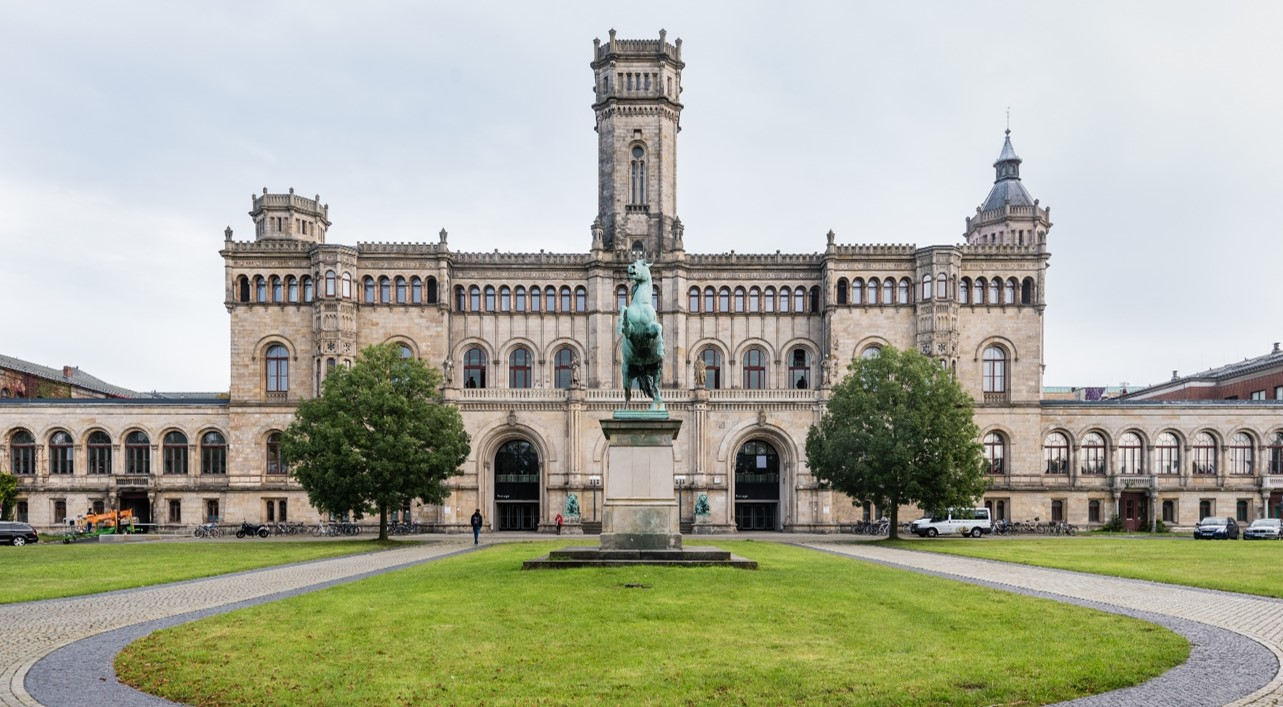
\includegraphics[width=0.65\textwidth]{figures/luh_default_presentation_title_image.jpg}}

% Title page: luhstyle
% \setbeamertemplate{title page}[luhstyle]
% % Add optional title image here
% \addtitlepageimage{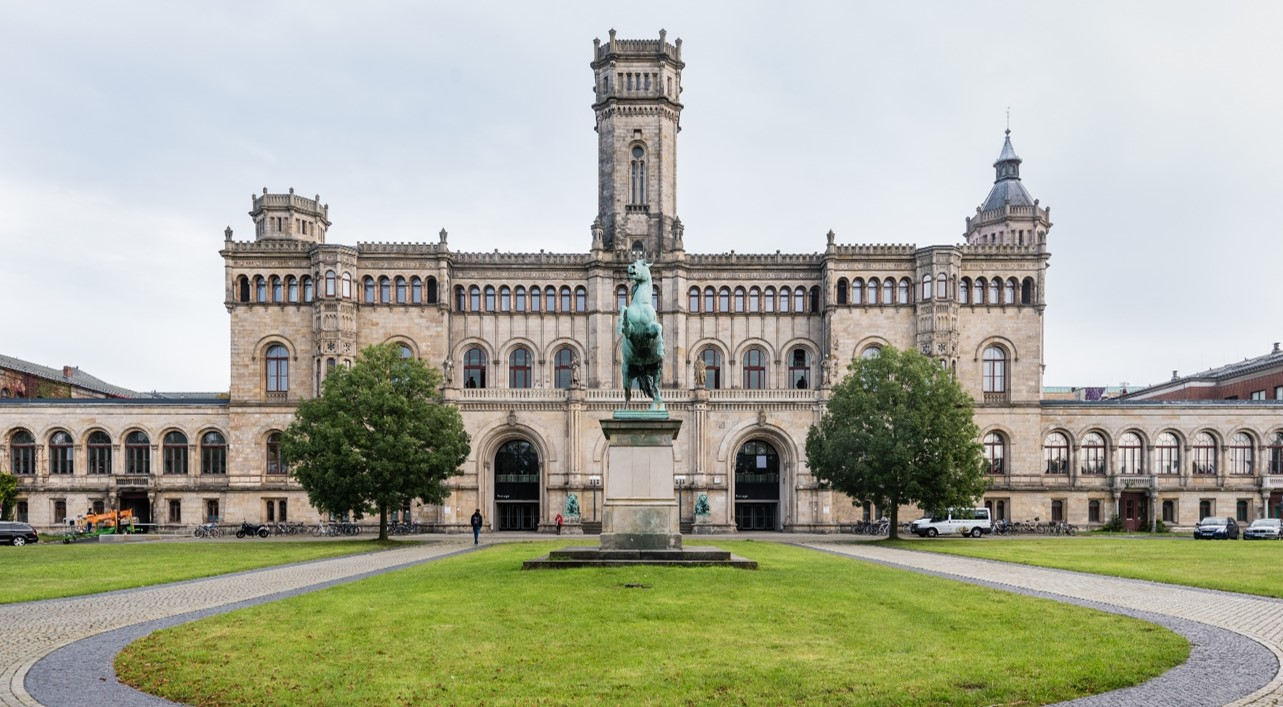
\includegraphics[width=0.75\textwidth]{figures/luh_default_presentation_title_image.jpg}}

\author[Abedjan \& Lindauer]{Ziawasch Abedjan \& Marius Lindauer\\[1em]
	
\includegraphics[height=\logoheight]{../latex_main/figures/luh_logo_rgb_0_80_155.pdf}\qquad
	
\includegraphics[height=\logoheight]{../latex_main/figures/DBIS_Kurzlogo.png}\qquad

\includegraphics[height=\logoheight]{../latex_main/figures/TNT_darkv4}\qquad

\includegraphics[height=\logoheight]{../latex_main/figures/L3S.jpg}	}
\date{Summer Term 2022; \hspace{0.5em} {
\includegraphics[height=1.5em]{../latex_main/figures/Cc-by-nc-sa_icon.svg.png}}; based on \href{https://ds100.org/fa21/}{[DS100]}
}


%%% Custom Packages
%----------------------------------------------------------------------
% Create dummy content
\usepackage{blindtext}

% Adds a frame with the current page layout. Just call \layout inside of a frame.
\usepackage{layout}


%%% Macros
%\renewcommand{\vec}[1]{\mathbf{#1}}
% \usepackage{bm}
%\let\vecb\bm

\title[CV, Reg \& AutoML]{DS: Cross-Validation, Regularization \& AutoML}
\subtitle{Regularization}

\graphicspath{ {./figure/} }
%\institute{}


\begin{document}
	
	\maketitle
	\begin{frame}{Basic Idea}
	    \begin{equation*}
	        \hat{\theta} \in \argmin_{\theta} \frac{1}{n}\sum\limits_{i=1}^n\mathcal{L}(y_i,f_{\bm{\theta}}(\bm{x}_i))
	    \end{equation*}
	    \underline{such that:}
	    \begin{equation*}
	        f_\theta \text{ does not 'overfit'}
	    \end{equation*}
	    Can we make this more formal?
	\end{frame}
	
	
	\begin{frame}[c]{Basic Idea}
	    \begin{equation*}
	        \hat{\theta} \in \argmin_{\theta} \frac{1}{n}\sum\limits_{i=1}^n\mathcal{L}(y_i,f_{\bm{\theta}}(\bm{x}_i))
	    \end{equation*}
	    \underline{such that:}
	    \begin{equation*}
	         \text{Complexity}(f_{\bm{\theta}}) \leq \beta
	    \end{equation*}
	    Complexity: How do we define this?\\
	    $\beta$:  Regularization Hyperparameter

	\end{frame}
	
	
	\begin{frame}[c]{Idealized Notion of Complexity}
	   \begin{equation*}
	         \text{Complexity}(f_{\bm{\theta}}) \leq \beta
	    \end{equation*}
        \begin{itemize}
            \item Focus on complexity of linear models:
            \begin{itemize}
                \item Number and kinds of features
            \end{itemize}
            \item Ideal definition:
            \begin{equation*}
                \text{Complexity}(f_{\bm{\theta}}) = \sum\limits_{j=1}^d\mathbb{I}[\bm{\theta}_j \neq 0] 
            \end{equation*}
            \item Why?
        \end{itemize}
	\end{frame}
	
	
	\begin{frame}[c]{Ideal “Regularization”}
	Find the best value of $\theta$ which uses fewer than $\beta$ features.
	  \begin{equation*}
	        \hat{\theta} \in \argmin_{\theta} \frac{1}{n}\sum\limits_{i=1}^n\mathcal{L}(y_i,f_{\bm{\theta}}(\bm{x}_i))
	    \end{equation*}
	    \underline{such that}
	    \begin{equation*}
                \text{Complexity}(f_{\bm{\theta}}) = \sum\limits_{j=1}^d\mathbb{I}[\bm{\theta}_j \neq 0]  \leq \beta
        \end{equation*}
        Combinatorial search problem – NP-hard to solve in general.

	\end{frame}
	
	\begin{frame}{Different Norms for Regularization}
	
	\begin{center}
	       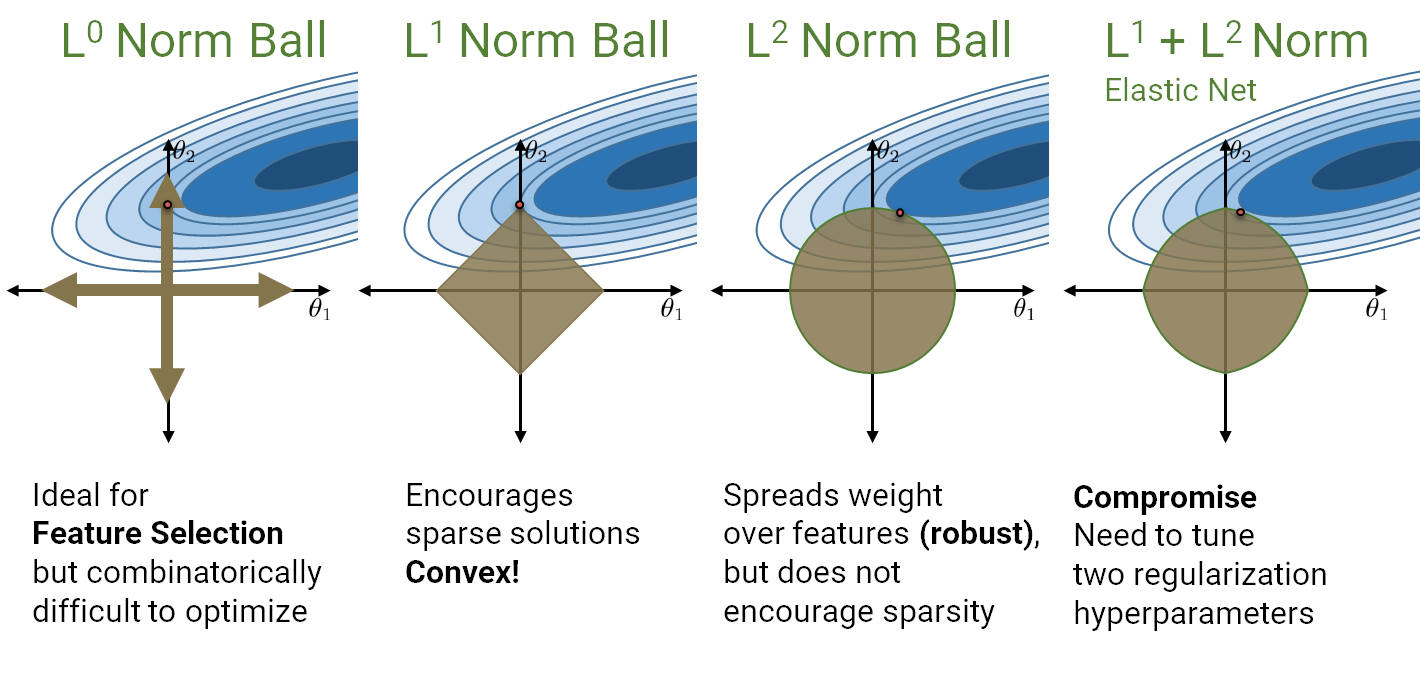
\includegraphics[scale=.3]{Bild17}
	       
	       $L^0 = \sum_{j=1}^d\mathbb{I}[\bm{\theta}_j \neq 0]$\hspace{1em} $L^1 = \sum_{j=1}^d|\bm{\theta}_j|$\hspace{1em} $L^2 = \sum_{j=1}^d\bm{\theta}_j^2$
	\end{center}
	    
	\end{frame}
	
	\begin{frame}{Generic Regularization}
	    
	    \begin{columns}
	            
	            \begin{column}{0.5\textwidth}
	                
	                Constrained:
	                	    \begin{align*}
                    	        &\text{Complexity}(f_{\bm{\theta}}) = R(\bm{\theta})\\
                    	        &\hat{\theta} \in \argmin_{\theta} \frac{1}{n}\sum_{i=1}^n\mathcal{L}(y_i,f_{\bm{\theta}}(\bm{x}_i))\\
                    	        &\underline{\text{such that: }} R(\bm{\theta}) \leq \beta
                    	    \end{align*}
	                
	            \end{column}
	            
	            \begin{column}{0.5\textwidth}
	            
	                Unconstrained (obtained by Lagrangian duality):
	                
	                	    \begin{align*}
	        &\text{Complexity}(f_{\bm{\theta}}) = R(\bm{\theta})
	    \end{align*}
	    \begin{equation*}
	        \hat{\theta} \in \argmin_{\theta}\left[ \left(\frac{1}{n}\sum_{i=1}^n\mathcal{L}(y_i,f_{\bm{\theta}}(\bm{x}_i)) \right) + \lambda R(\bm{\theta})\right]
	    \end{equation*}
        $\lambda$: Regularization Hyperparameter
	                
	                
	            \end{column}
	            
	    \end{columns}

	\end{frame}
	
	
	
	\begin{frame}{Standardization and the Intercept Term}
	    \begin{itemize}
	        \item Height = $\theta_1 \cdot$  (age\_in\_seconds) + $\theta_2\cdot$ (weight\_in\_tons)
	    \end{itemize}
	    $\theta_1$ will be small (because lives on a large scale)  and  $\theta_2$ will be large (because lives on a small scale)
	    \begin{columns}
	        \begin{column}{.5\textwidth}
	                \begin{itemize}
	                    \item \alert{Regularization penalizes dimensions equally}
	                    \item Standardization
	                    \begin{itemize}
	                        \item Ensure that each dimensions has the same scale
	                        \item centered around zero
	                    \end{itemize}
	                    \item Intercept Terms
	                    \begin{itemize}
	                        \item Typically don’t regularize intercept term 
	                    \end{itemize}
	                \end{itemize}
	        \end{column}
	        
	        \begin{column}{.4\textwidth}
	                \\ 
	                Standardization\\
	                For each dimension $k$:
	                \begin{equation*}
	                    Z_k = \frac{x_k - \mu_k}{\sigma_k}
	                \end{equation*}
	        \end{column}
	    \end{columns}
	\end{frame}
	
\end{document}